\documentclass{beamer}
\usepackage[latin1]{inputenc}
\usepackage{graphics}
\usepackage{amsfonts}
\usetheme{Warsaw}
\title[CS 626 : Project Presentation]{Private Anonymous Messaging \\With Friends!}
\author{Ruchith Fernando}
\institute{Purdue University}
\date{April 26, 2011}
\begin{document}

\begin{frame}
\titlepage
\end{frame}


\begin{frame}{Problem}
\begin{itemize}
\item A user wants to send a message to all his current contacts
\item Even if they are \textbf{offline!}
\item \textbf{Only} trusts his/her immediate contacts
\item A contact can re-distribute messages on requests
\end{itemize}
\end{frame}


\begin{frame}{Problem}
\begin{figure}
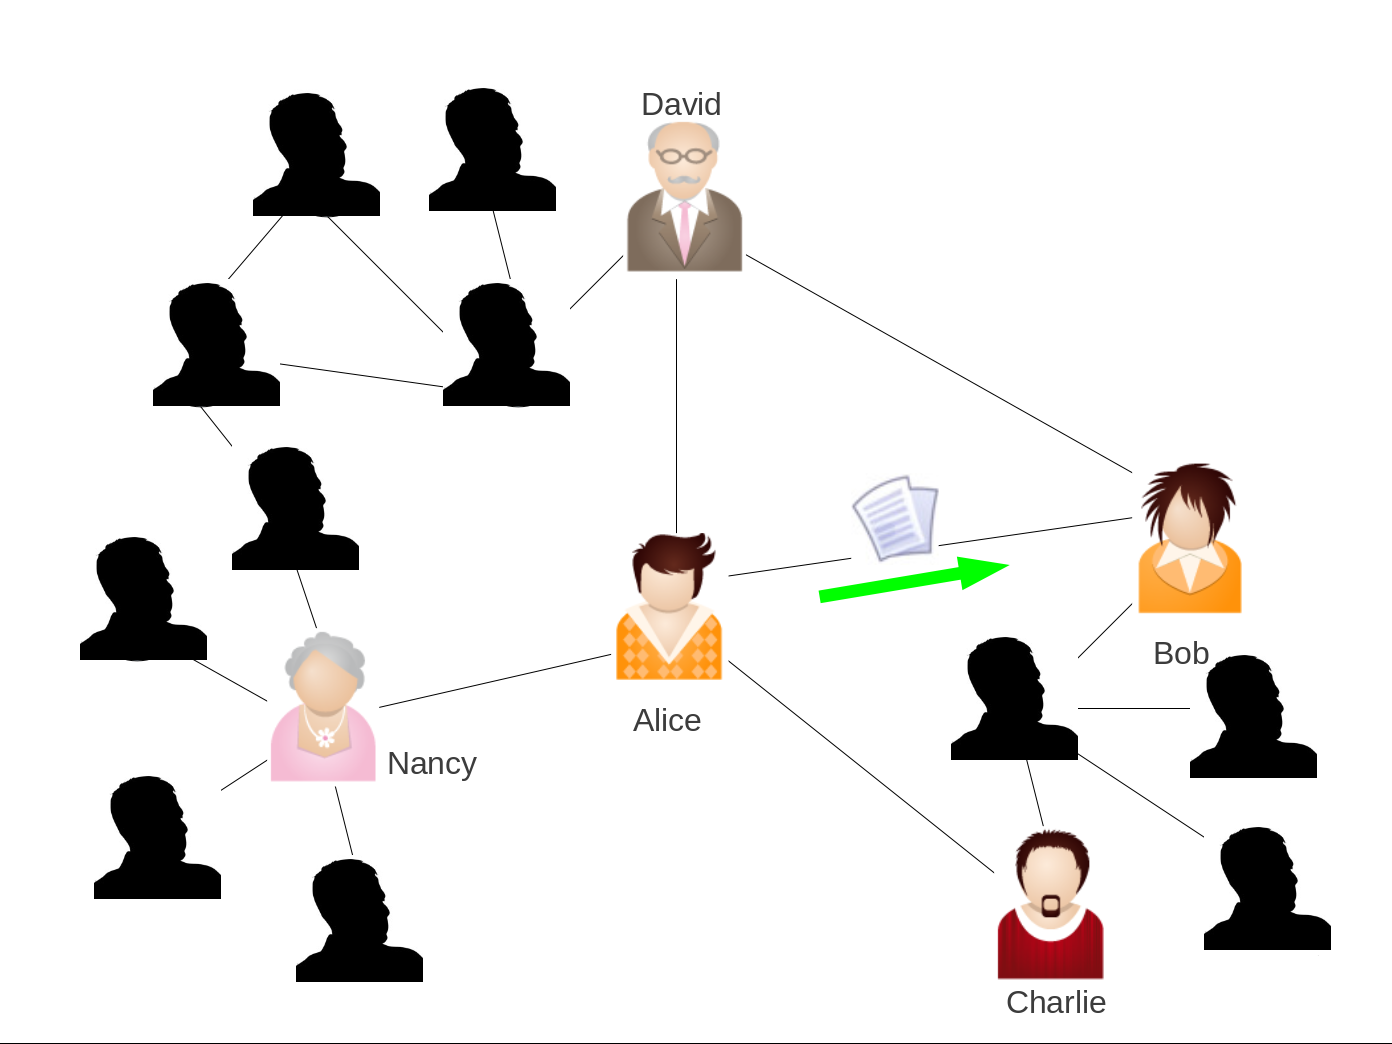
\includegraphics[height=6cm]{img/img1.png} 
\end{figure}
\end{frame}


\begin{frame}{Problem}
\begin{figure}
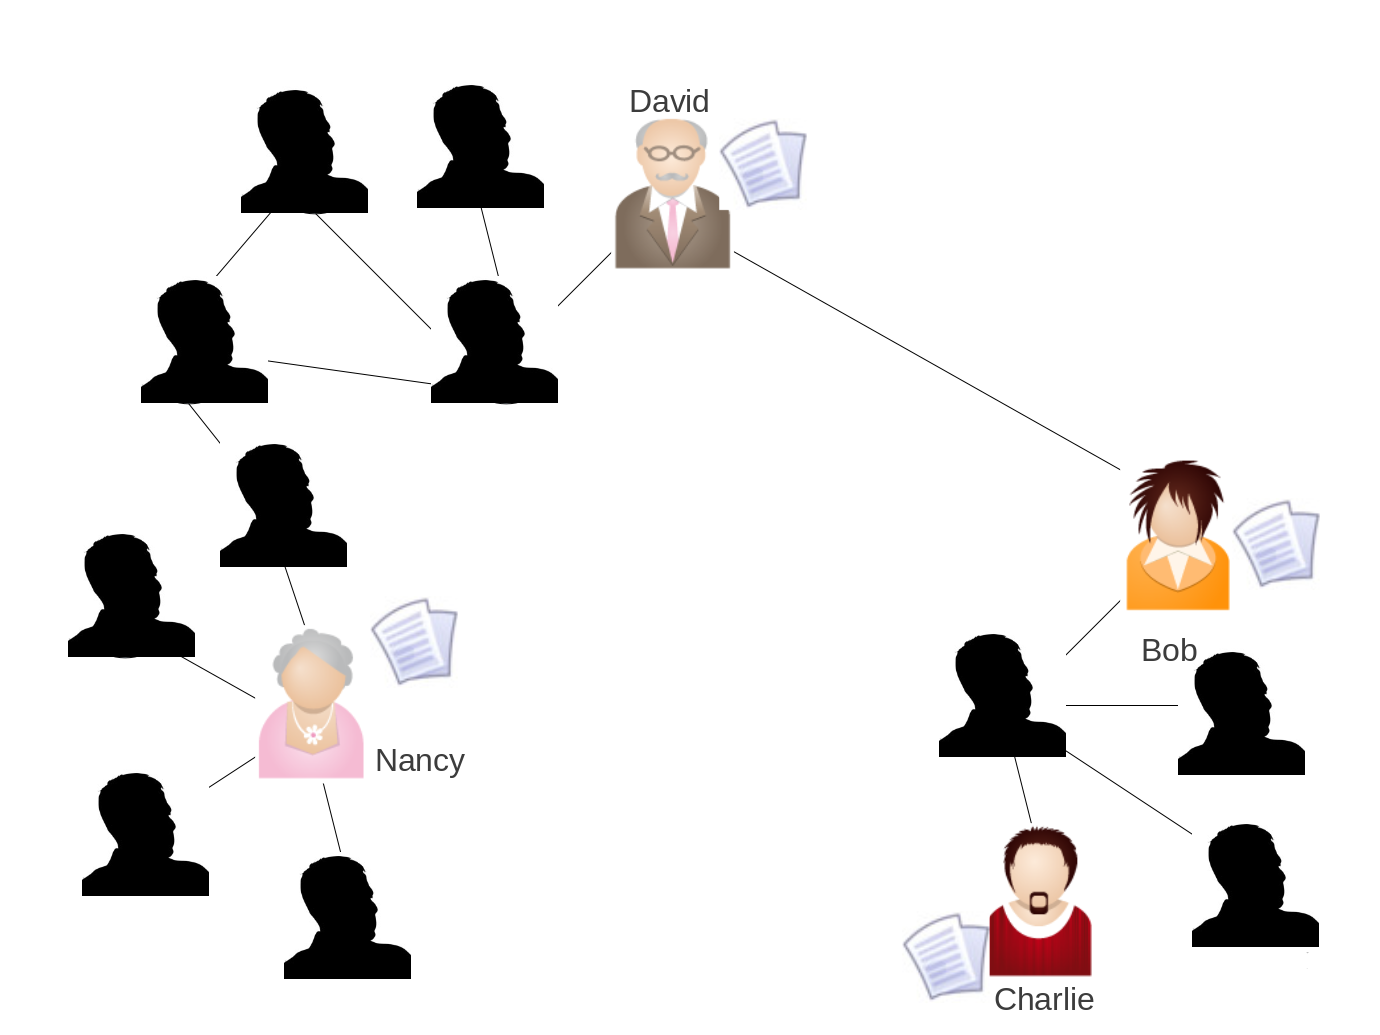
\includegraphics[height=6cm]{img/img2.png} 
\end{figure}
\end{frame}

\begin{frame}{Proposed Solution}
\begin{itemize}
\item Modify HIBE (Hierarchical Identity Based Encryption with
Constant Size Ciphertext, Boneh et.al)
\item Each contact is issued a private key (only private channel for key exchange)
\item Contacts generate \textbf{anonymous} public keys using their private keys
\item Broadcast update request to be processed by other contacts 
\item Re-key mechanism with \textbf{public} data (no private channel requirement)
\end{itemize}
\end{frame}

\begin{frame}{Hierarchical Identity Based Encryption}
\begin{figure}
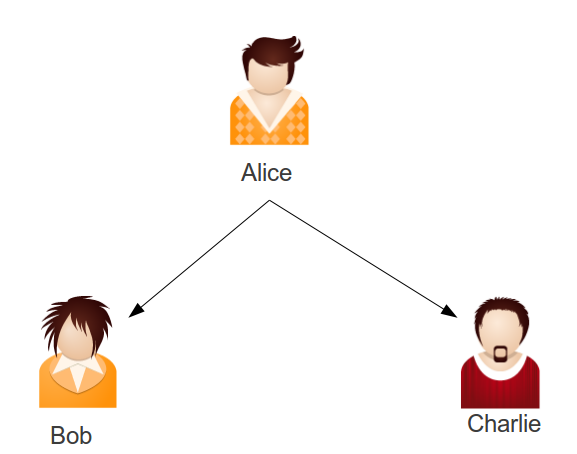
\includegraphics[height=3cm]{img/img3.png} 
\end{figure}
\pause \begin{itemize}
\item Identities:
 \begin{itemize}
	\item Alice: $I_1$
	\item Bob: $I_1,{I_2}_1$
	\item Charlie: $I_1,{I_2}_2$
\end{itemize}
\pause \item $e : \mathbb{G} \times \mathbb{G} \to \mathbb{G}_1 , |\mathbb{G}| = p$
\pause \item $params = (g, g_1, g_2, g_3, h_1, h_2) ,  g_1 = g^\alpha , \alpha \in \mathbb{Z}_p$
\pause \item $mk = {g_2}^\alpha$
\end{itemize}
\end{frame}

\begin{frame}{Hierarchical Identity Based Encryption}
\begin{figure}
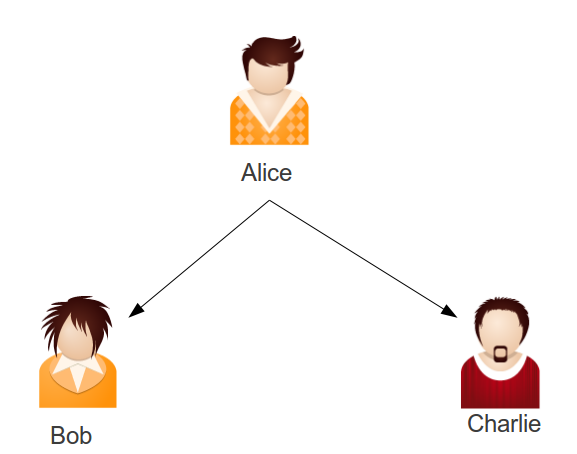
\includegraphics[height=3cm]{img/img3.png} 
\end{figure}

\begin{itemize}
\item Alice :
\begin{itemize}
\item ${K_{priv}}_{alice} = KeyGen(I_1, params, mk)$ 
\item ${K_{pub}}_{alice} = I_1$
\end{itemize}

\item Bob :
\begin{itemize}
\item ${K_{priv}}_{bob} = KeyGen(I_1, I_2, params, {K_{priv}}_{alice})$
\item ${K_{pub}}_{bob} = I_1, {I_2}_1$
\end{itemize}

\item To encrypt for Bob \\ $CT = Encrypt(msg, I_1, {I_2}_1, params)$


\end{itemize}
\end{frame}

\begin{frame}{Changes to HIBE}

\begin{itemize}
\item Update $Encrypt()$ to work with ${h_1}^{I_1}{h_2}^{{I_2}_1} = ID$
\item To encrypt for Bob \\ $CT = Encrypt'(msg, ID, params)$
\item On re-key update $\alpha$ and only generate minimum public data for existing contacts.
\end{itemize}
\end{frame}

\begin{frame}{Usage}
\begin{itemize}
\item First level identity ($I_{r_1}$) and private key to a contact
\item A contact issue him/herself a second level identity with a random $I_{r_2}$
\item Broadcsts a request for data ($<$\emph{user}, $ID_r>$) where $ID_r = {h_1}^{I_{r_1}}{h_2}^{I_{r_2}}$
\item Any other contact of the \emph{user} can respond to the request, by encrypting with $params_{user}$ : \\\
$CT = Encrypt'(msg, ID_r, params_{user})$
\end{itemize}
\end{frame}

\begin{frame}{Usage : Revocation}
\begin{itemize}
\item If the \emph{user} removes a contact
\item Re-key :
\begin{itemize}
\item $params_{user}$ update 
\item A public component of the current contacts' private keys
\item Indexed by blinded $ID_{contact}$
\end{itemize}
\end{itemize}
\end{frame}


\begin{frame}{Implementation}
\begin{itemize}
\item http://code.google.com/p/anon-encrypt/
\item Using Java Pairing Based Cryptography Library (JPBC)\footnote{http://gas.dia.unisa.it/projects/jpbc/}
\item Implemented as a library
\item Demo application
\end{itemize}
\end{frame}

\begin{frame}{Demonstration}
\Huge{DEMO!}
\end{frame}

\end{document}
